\DiaryEntry{Semidefinite Relaxation}{2016-09-27}{Optimization}

\subsection{Problem}

Original paper \href{\%7Bfilename\%7D/files/sdrapp-SPM.pdf}{here}, an
interesting presentation
\href{\%7Bfilename\%7D/files/20120616101847.pdf}{here}.

We want to solve the following minimization problem


\begin{align*}
\min & x^T C x \\
s.t. & x^T F_i x \geq g_i, \quad i=1,\ldots,p \\
     & x^T H_i x = l_i, \quad i=1,\ldots,m
\end{align*}


All matrices \(C, F_i, H_i\) are symmetric \(n \times n\) matrices and \(x\) is a length-n vector. This is a quadratically constrained quadratic problem (QCQP) and - in general - non-convex. As an example how the constraints may look like consider

\[ F_1 = 
\begin{pmatrix}
2 & 2 \\
2 & 3
\end{pmatrix}, F_2 = 
\begin{pmatrix}
2 & -3/2 \\
-3/2 & 3
\end{pmatrix}
\]

with \(g_1 = g_2 = 10\).

\begin{figure}[H]
\centering
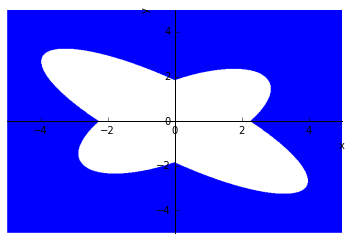
\includegraphics{images/sdr_1.png}
\end{figure}

The blue region is the feasible region and is clearly not convex. The objective function has elliptical contour lines (centered at the origin) which may arbitrarily rotated with respect to the axis (depending on the matrix \(C\)).

\subsection{Solution}

We can rewrite the problem by substituting \(X = x x^T\) and obtain


\begin{align*}
\min \,\, & \text{tr} (C X) \\
s.t. & \text{tr} (F_i X) \geq g_i, \quad i=1,\ldots,p \\
     & \text{tr} (H_i X) = l_i, \quad i=1,\ldots,m \\
     & X \succeq 0, \text{rank}(X) = 1
\end{align*}


The problem has now a linear objective function, linear constraints, the psd condition on \(X\) is also not hard, but the rank-1 condition on \$X" \textbf{is} hard. This comes at no surprise as a substitution cannot convert an NP-hard problem into an easy one.

The key idea is to drop the rank-1 condition and arrive at the semidefinite relaxation


\begin{align*}
\min \,\, & \text{tr} (C X) \\
s.t. & \text{tr}(F_i X) \geq g_i, \quad i=1,\ldots,p \\
     & \text{tr}(H_i X) = l_i, \quad i=1,\ldots,m \\
     & X \succeq 0
\end{align*}


This problem is convex and can be solved with standard methods quite
easily. However, the solution will typically not be a rank-1 matrix and
the question is how to find the solution of the original problem.
According to the paper, this is ``problem-specific''; e.g.~simple
methods like an EVD of \(X\) and cutting off all eigenvalues except the
largest one, or randomization methods are mentioned.

\subsection{Example}

As an example consider solving

\begin{align*}
\min \,\, & \text{tr} (X) \\
s.t. & \text{tr}(F X) \geq 15 \\
     & X \succeq 0, \text{rank}(X) = 1
\end{align*}

with

\[
F = \begin{pmatrix} 2 & 2 \\ 2 & 3 \end{pmatrix}
\]

The constraint $\text{tr}(F X) \geq 15$ has the following form

\begin{figure}
\centering
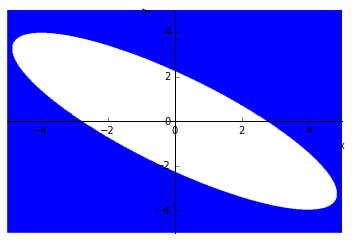
\includegraphics{images/sdr_2.png}
\end{figure}

The contour plot of the objective function are just concentric circles with center at the origin. Wit geometric intuition, the solution of the problem is therefore the intersection of the ellipse's minor axis with the ellipse: Tis point is feasible and has minimum distance from the origin (and therefore the objective function minimal).

We can solve this with the following cvxpy script

\begin{verbatim}
import cvxpy as cvx
import numpy as np

X = cvx.Semidef(2)
F = np.array([[2, 2], [2, 3]])
constraints = [ cvx.trace(F*X) > 15]

# Form objective.
obj = cvx.Minimize(cvx.trace(X))

# Form and solve problem.
prob = cvx.Problem(obj, constraints)
prob.solve()  # Returns the optimal value.
print("status:", prob.status)
print("optimal value", prob.value)
print("optimal var", X.value)

# finding a 2-d point by using a rank-one approximation
d, u = np.linalg.eigh(X.value)
print("rank-1 approx:", np.sqrt(d[1])*u[:,1])
\end{verbatim}

which yields

\begin{verbatim}
rank-1 approx: [[ 1.11597753] [ 1.42931817]]
\end{verbatim}

Here we have used an EVD of the solution \(X\) and then take the vector corresponding to the largest eigenvalue as approximation of the original non-convex problem.

The ellipse minor axis can be found using an EVD on \(F\) which yields for the minor axis

\begin{verbatim}
array([ 0.61541221,  0.78820544])
\end{verbatim}

This is the direction of the minor axis. Let's call the slope \(\alpha = \frac{0.788\ldots}{0.615\ldots}\). The line of the minor axis in parametric form is therefore \(x = t, y = \alpha t\). The constraint is given by \(2x^2 + 3y^2 + 4xy = 15\). We seek the intersection point of line and ellipse which is obtained as

\[
2t^2 + 3\alpha^2 t^2 + 4 \alpha t^2 = 15 \rightarrow t = \sqrt{\frac{15}{2 + 4 \alpha + 3 \alpha^2}}
\]

From this value we have \(x_o =1.12, y_o = 1.43\). This value matches the result given by cvxopt (and subsequent rank-1 approximation).
